
\section{Results}
\label{sec:results}

\subsection{The Output Plot}
\label{sub:output}

\begin{figure}[tb]
	\centering
	\includegraphics[width=\columnwidth]{./output/run-pespread/pespread_0.01/n1/graph.pdf}
	\caption{
		Blue line representing the reconstruction of the shape of the beam that
		hits the screen consistently overestimates the vertical beam size. This
		run used a small percentage energy spread of \SI{1}{\percent}. With all
		other parameters set to their expected value.
	}
	\label{fig:yoverestimate}
\end{figure}

Along with the \(\chi^2\) minimised parameter values of the fit, each simulation
generated a plot, showing the simulated, measured and fitted vertical beam size
functions as a function of horizontal position \(x\) on the screen.
Figure~\ref{fig:yoverestimate} is an output plot for a run with a small
(\SI{1}{\percent}) energy spread. The solid black line is the shape of the
simulated electron beam that hits the screen, the black points show the
simulated measurements of the RMS width of the fitted gausian for each vertical
strip of pixels. The blue dashed line is the beam size function fitted to the
points.

\subsection{Binning errors}

After the investigation of multiple experimental parameters, the emittance
measurement consistently converged to a value \num{1e-8} larger than the input
emittance. The reason for this systematic error was found to be due to the
discritisation of the beam hitting the screen meaning that the measurement of
the vertical beam size was consistently overestimated. Since the electrons in
each pixel are not uniformly distributed but rather more densely distributed
closer towards the mean value, giving rise to a systematic overestimation of the
vertical beam size of up to two times the vertical size of the pixel. This
effect can be seen most clearly when a very small energy spread was used as can
be seen in Figure~\ref{fig:yoverestimate}, where the measured beam heights are
consistently larger than the actual beam height.

\subsection{Energy Spread}

\begin{figure*}[!tb]
	\centering
	\begin{subfigure}[t]{\columnwidth}
		% 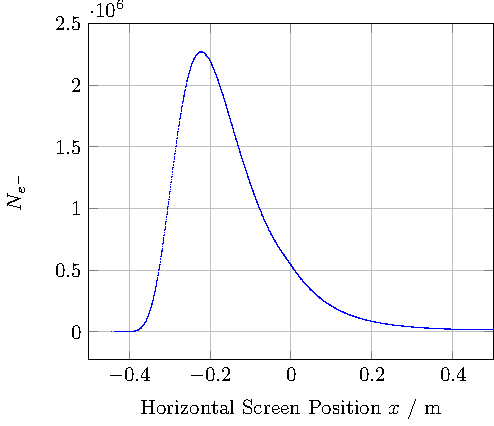
\includegraphics[width=1\linewidth]{./figures/edist.pdf}
		\includegraphics{./output/run-pespread/emit_vs_pespread.pdf}
		\caption{
			Plot of the simulated emittance measurement against the percentage
			spread of beam energy.
		}
		\label{fig:emit_pespread}
	\end{subfigure}\hfill~
	\begin{subfigure}[t]{\columnwidth}
		% 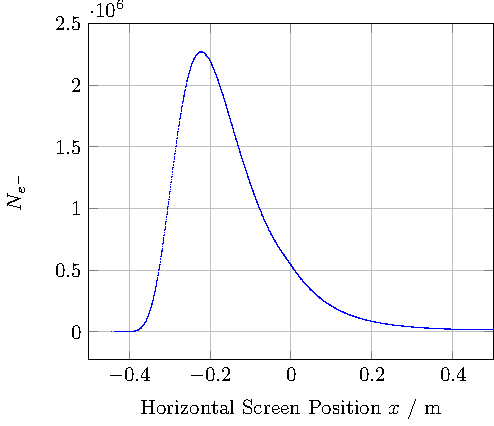
\includegraphics[width=1\linewidth]{./figures/edist.pdf}
		\includegraphics{./output/run-pespread/emitperr_vs_pespread.pdf}
		\caption{
		}
		\label{fig:emitperr_pespread}
	\end{subfigure}
\end{figure*}


Initially, the mean energy of the beam and energy spread of the beam were tested
independently. Simulations for all combinations of the following energies \(E
\in \left\{ 0.5, 1, 1.3, 2.0, 3.0 5.0\right\} \) and the following energy
spreads \(\sigma_E \in \left\{ 0.01, 0.1, 0.3, 0.4 \right\}\) were run.  These
energies and energy spreads were chosen such that at least one standard
deviation of the beam hit the screen. As Figure~\ref{fig:eofx} shows, the range
of energies that hit the screen for the is from
\SIrange{\sim0.28}{6}{\giga\electronvolt}.

The estimated energy spread of the electron beam is
\SI{0.4}{\giga\electronvolt}, 
% TODO dipole adjustable so could have larger energies
% TODO still need to investigate upper range



It was found that the error of the measurement of the emittance 
% TODO oh god this was the wierd one

Mean beam energies tested ranged from \SIrange{0.1}{4}{\giga\electronvolt}

\subsection{Input Emittance}

\begin{figure*}[!tb]
	\centering
	\begin{subfigure}[t]{\columnwidth}
		\centering
		\includegraphics{./output/run-inemit/emitr_vs_inemit.pdf}
		\caption{
		}
		\label{fig:emitr_inemit}
	\end{subfigure}%
	~
	\begin{subfigure}[t]{\columnwidth}
		\centering
		\includegraphics{./output/run-inemit/emitrperr_vs_inemit.pdf}
		\caption{
		}
		\label{fig:emitrperr_inemit}
	\end{subfigure}%
\end{figure*}

\begin{figure}[!tb]
	\centering
	\includegraphics[width=\columnwidth]{./output/run-inemit/emit_7e-5/n1/graph.pdf}
	\caption{
		Beam reconstruction for an input emittance of \num{7e-5} showing the
		underestimation of the measured vertical beam sizes.
	}
	\label{fig:large_emit}
\end{figure}


Since the emittance 

\subsection{Background Photons}


\begin{figure*}[!t]
	\centering
	\begin{subfigure}[t]{\columnwidth}
		\centering
		\includegraphics{./output/run-bgdens/emit_vs_bgdens.pdf}
		\caption{
		}
		\label{fig:emit_bgdens}
	\end{subfigure}%
	~
	\begin{subfigure}[t]{\columnwidth}
		\centering
		\includegraphics{./output/run-bgdens/emitperr_vs_bgdens.pdf}
		\caption{
		}
		\label{fig:emitperr_bgdens}
	\end{subfigure}%
\end{figure*}

\begin{figure}[!tb]
	\centering
	\includegraphics[width=\columnwidth]{./output/run-bgdens/bgphotons_1e4/n6/graph.pdf}
	\caption{
		Beam reconstruction for a large background.
	}
	\label{fig:large_bg}
\end{figure}



